\section{Mixed Criticality Architectures}

%%%%%%%%%%%%%%%%%%%%%%%%%%%%%%%%%%%%%%%%%
% \begin{frame}{Integrated Dependable Architecture for Many-Cores}

% \begin{itemize}
% \item Resources are distributed over Tiles, which are groups of resources sharing one NoC access point
% \item Tiles communicate with each other through an Address Translation Table
% \item A budgeting mechanism limits the number of messages sent to each local address
% \item One special tile serves as System Controller
% \begin{itemize}
% \item The SC is responsible for ATT configuration
% \item The SC can stall, reset, or disable any tile
% \end{itemize}
% \end{itemize}

%\end{frame}

\begin{frame}{Integrated Dependable Architecture for Many-Cores}

\begin{center}
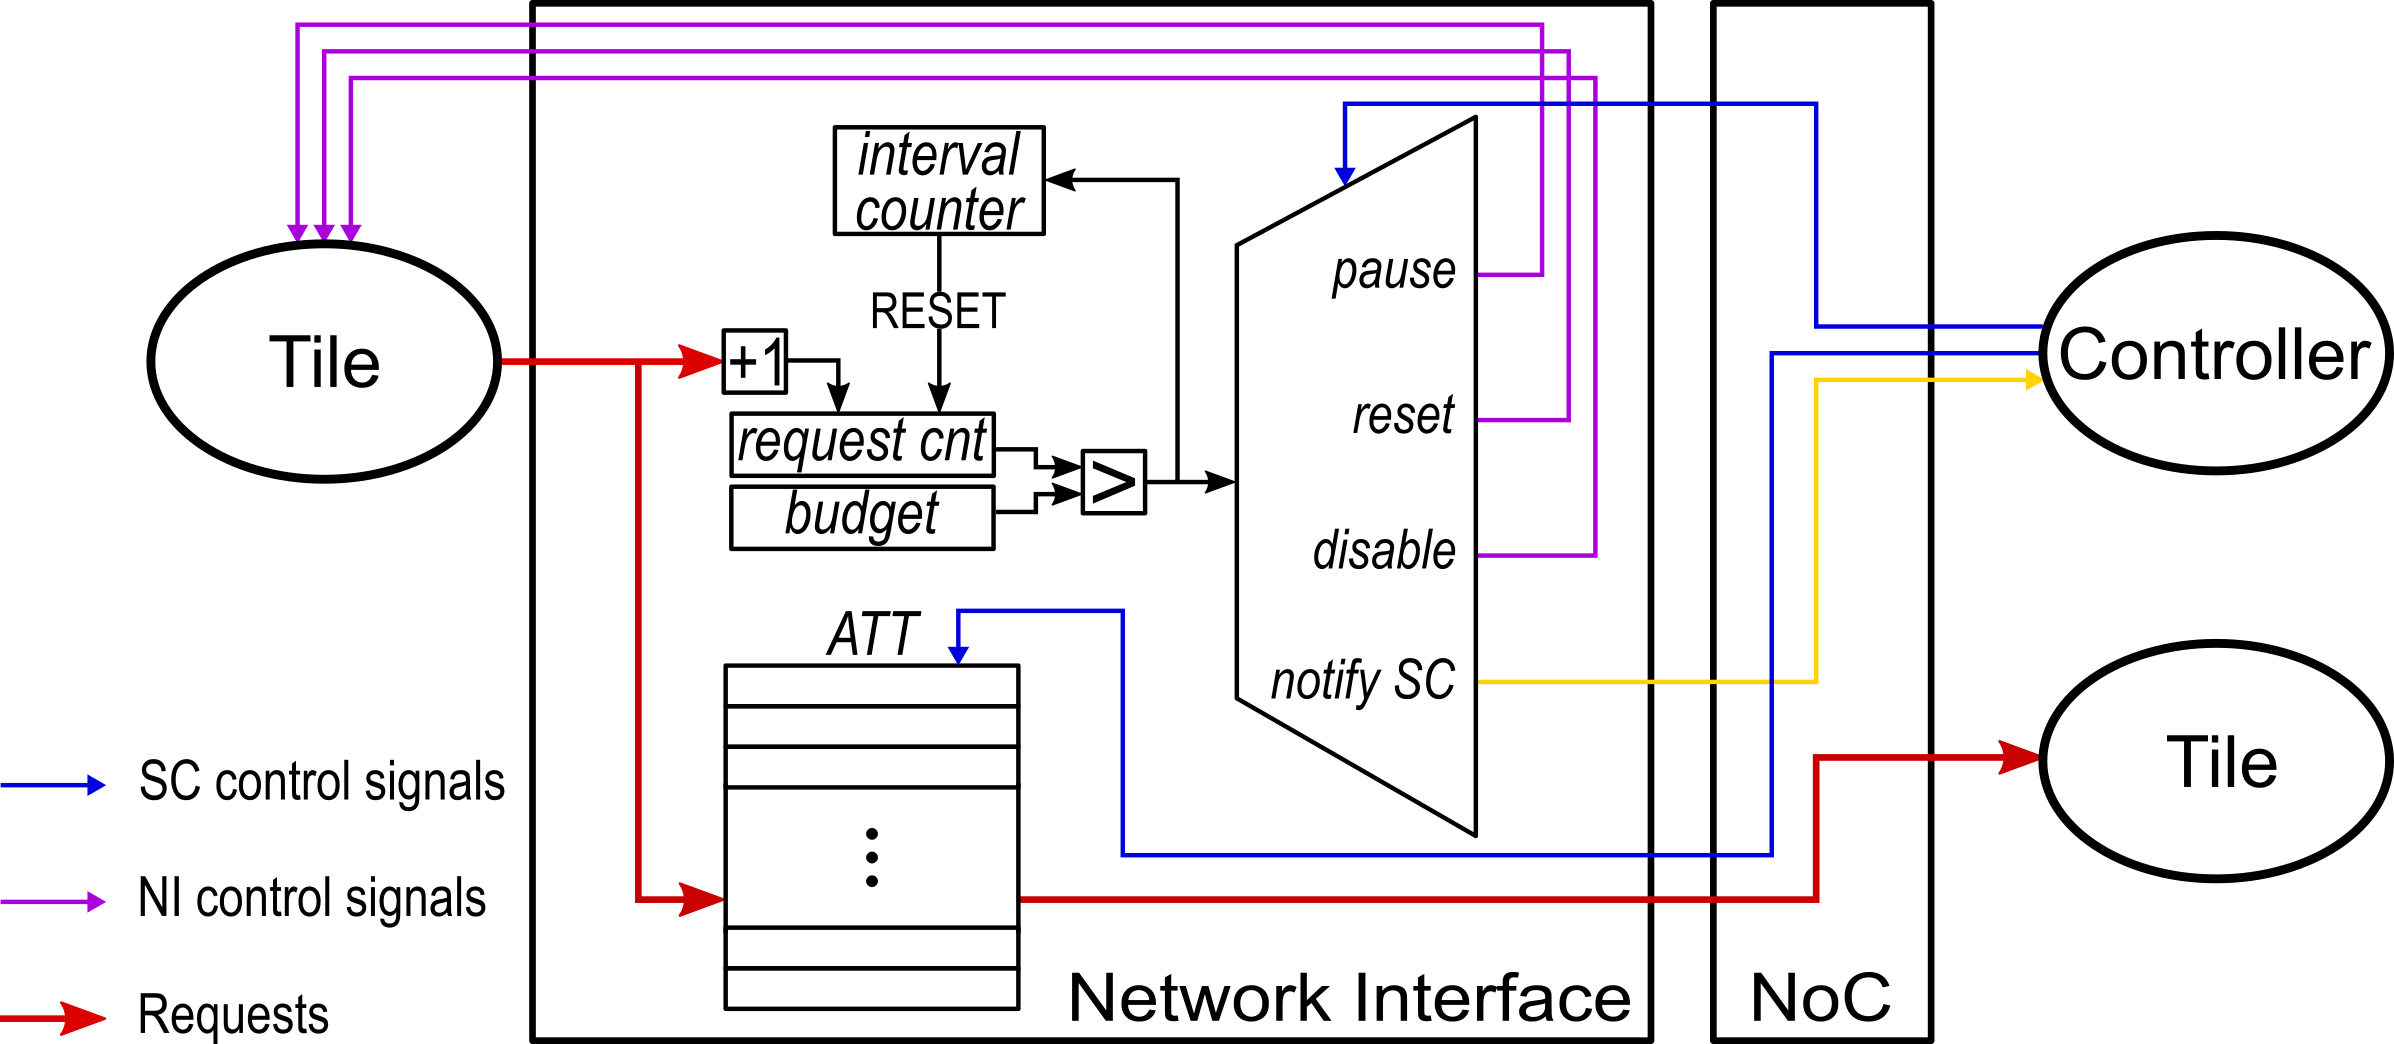
\includegraphics[width=\textwidth]{IDAMC.png}
\end{center}

\end{frame}
%%%%%%%%%%%%%%%%%%%%%%%%%%%%%%%%%%%%%%%%%
\begin{frame}{Integrating Scheduling and Data mapping}

Hardware model:

\begin{itemize}
\item \visible <1-> {16 Clusters}
\item \visible <2-> {Each containing 16 cores, 3 NoC interfaces, and 16 SRAM banks}
\item \visible <3-> {Each SRAM bank has its own dedicated controller, which arbitrates between all cores and interfaces}
\visible <4-> {
\begin{itemize}
\item NoC receiver interface always has priority
\item RR arbitration is performed between other components
\end{itemize}}
\end{itemize}

\end{frame}

\begin{frame}{Integrate Scheduling and Data mapping}

Software model:

\begin{itemize}
\item \visible<1-> {Independent task set and scheduler for each cluster}
\item \visible<2-> {Criticality mode switch}
\item \visible<3-> {Scheduling data:
\begin{itemize}
\item Execution times \textbf{without memory accesses}
\item Number of memory accesses
\item Dependency graph
\end{itemize}}
\item \visible<4-> {Tasks of different criticality cannot be scheduled on the same time frame}
\item \visible<5-> {Joint computation of task schedule and data mapping to SRAM banks}

\end{itemize}
\end{frame}

\begin{frame}{Controlling interference from other tiles}

When a task requires data to be fetched through the NoC

\vspace{1cm}

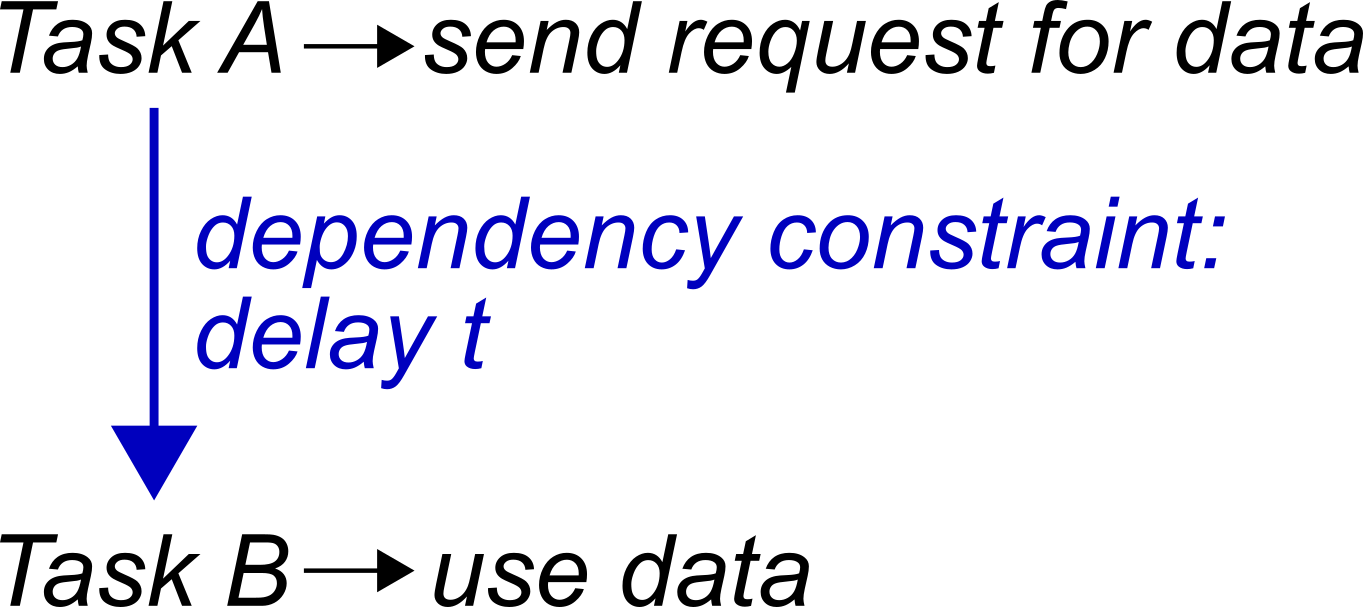
\includegraphics[width=0.5\textwidth]{initDataFetch.png}

\vspace{0.5cm}

\(t = 2* \text{NoC worst-case latency} + \text{resource worst-case response time}\)

\end{frame}

\begin{frame}{Higher level modeling - Resource Servers}
\begin{itemize}
\item \visible <1-> {A resource server "encapsulates" the access to a resource}
\item \visible <2-> {This can allow to consider only the server and the requesting component in modeling}
\item \visible <3-> {The resource itself and the interfering components can be laid aside \textbf{provided the inter-process communication protocol is adequate}}
\item \visible <4-> {For MCS, the IPC protocol should also take criticality into account}
\end{itemize}
\end{frame}

\begin{frame}{Resource Server for MCS}

\includegraphics<1>[width=\textwidth]{ResourceServerGrey.png}
\includegraphics<2>[width=\textwidth]{ResourceServerGrey2.png}
\includegraphics<3>[width=\textwidth]{ResourceServer.png}

\end{frame}
%%% Local Variables:
%%% mode: latex
%%% TeX-master: "slides"
%%% End:
